\documentclass[12pt]{article}
\usepackage[margin=1.0in]{geometry}

%\usepackage[utf8]{inputenc}
%\usepackage[T1]{fontenc}
%\usepackage{fixltx2e}
%\usepackage{longtable}
%\usepackage{float}
%\usepackage{wrapfig}
%\usepackage{rotating}
%\usepackage[normalem]{ulem}
%\usepackage{textcomp}
%\usepackage{marvosym}
%\usepackage{wasysym}
%\tolerance=1000

\usepackage{graphicx}
\usepackage{amsmath}
\usepackage{amssymb}
\usepackage{amsfonts}
\usepackage{bm}
\usepackage{algpseudocode}
\usepackage{hyperref}

\usepackage{listings}

\lstset{language=C}
\newcommand{\pd}[2]{\frac{\partial #1}{ \partial #2}}
\renewcommand{\v}[1]{\bold{#1}}

\title{CS 598 Final Project}
\author{Scott High and Erin Molloy}
\date{\today}


\begin{document}

\maketitle

\section{Introduction}
Molecular dynamics (MD) simulations are important for researching physical phenomena 
such as, the electronic structure of metal and the folding trajectories of proteins. 
In our final project, we will create performance expectations for a molecular dynamics 
simulation mini-app, called \href{https://github.com/exmatex/CoMD}{\texttt{CoMD}}, which is designed to expose the core features 
of molecular dynamics simulations in a code base that is simple to understand and modify.

% Outline contributions

%In our final project, we will create performance expectations for the Lennart-Jones(LJ) model 
%of potential energy. We propose to
%\begin{itemize}
%    \item [1] Create a performance expectation based on memory access patterns.
%    \item [2] Create a performance expectation of scalability based on communication.
%    \item [3] Attempt to improve performance and scalability.
%    \item [4] Compare the scalability of the Lennart-Jones model to that of the Embedded Atom Model.
%\end{itemize}

\subsection{Background}
Molecular dynamics simulations model the movement of individual particles over time. 
Particle motion is determined by Newton's well-known equation of motion, $F = ma$. 
In an $N$-particle simulation, the force on the particle at position 
$\bm{r}_i = (x_i, y_i, z_i)$ is given by
\begin{equation*}
    F_i = m_i \ddot{\bm{r}}_i = -\frac{\partial}{\partial \bm{r}_i} U(\bm{r}_1, \dots, \bm{r}_N)
\end{equation*}
The system of first order ODEs is integrated to find the position of particles at each time step.
Both the LJ and EAM models utilize inter-particle interactions or ``pair potentials''
within a predefined region of interaction.


% Compilation requires only a valid \texttt{C} compiler and a working \texttt{MPI} implementation.
% The code is relatively short, only a few thousand lines, and is extensively documented. 

\section{Performance Baseline}
% Erin Molloy

Detailed code timings are already built into \texttt{CoMD}. 



%
% 
%
%We will run performance
%experiments with the provided model of copper atoms in a lattice.

%
% 
%
\subsection{Single processor}
A performance baseline is obtained by running \texttt{CoMD} on a single processor.
and the size of the lattice by a factor of 10 in each dimension.


We will examine problem sizes larger than the size of the L2 cache (2MB - 
\href{https://bluewaters.ncsa.illinois.edu/user-guide}{\texttt{Blue Waters User Guide}}).

\subsection{Strong scaling}

\subsection{Weak scaling}

\section{Performance model}
All analysis is done assuming a one-level cache model and
approximating read and write times as equal.  The constants used in
the performance expectations are determined by the clock rate and
\texttt{STREAM} benchmark results as measured on Blue Waters.

The equations we are calculating for each particle in computer variables are
\begin{align}
  E_{tot} &= \sum_{ij} U_{LJ}(r_{ij}) \\
  U_{LJ}(r_{ij}) &= 
  A\left(\frac{1}{r_{ij}}\right)^{6}\left\{ \left(\frac{1}{r_{ij}}\right)^{6} - 1 \right\} \\
  \notag\\
  \textbf{F}(r_{ij}) &= - U'_{LJ}(r_{ij})\hat{r}_{ij} \notag\\
      &=  24 \frac{\epsilon}{r_{ij}} \left\{ 2 \left(\frac{\sigma}{r_{ij}}\right)^{12}
              - \left(\frac{\sigma}{r_{ij}}\right)^6 \right\} \hat{r}_{ij} \notag\\
              &=  A \frac{1}{r_{ij}^2} \left(\frac{1}{r_{ij}}\right)^{6} \left\{ 2 \left(\frac{1}{r_{ij}}\right)^{6}
              - 1 \right\} \textbf{r}_{ij}
\end{align}
in a fully periodic domain. The total number of simulation particles
is $N$, and each particle has $n$ neighbors within
$r_c=r_{\text{cutoff}}$.

We develope our performance model by calculating the cost of updating
particle $i$ and its interaction with each of its $n$ neighbors
$j$. The cost is:
\begin{itemize}
\item[A)] 3 loads for particle $i$'s position
\item[B)] For each particle $j$ where $r_{ij}<r_c$
  \begin{enumerate}
    \item $3$ loads for particle $j$'s position
    \item 3 subtractions, 3 multiplications, 2 additions and 1 division to calculate $\frac{1}{r_{ij}^2}$ 
    \item 3 multiplications to calculate $\left(\frac{1}{r_{ij}^2}\right)^3=\left(\frac{1}{r_{ij}}\right)^6$
    \item 2 subtractions and 2 multiplications to calculate $U_{LJ}$ (1 subtraction is for cutoff potential)
    \item 3 multiplications and 1 subtraction to calclulate $F(r_{ij})$
    \item 3 multiplications and 3 additions to calculate and update $F_{x,y,z}$
  \end{enumerate}
\item[C)] 1 write to save $U_{LJ}$. (Assume we can save the $U_{LJ}(r_{ji})$ term for free)
\item[D)] 3 writes to save $F_{x,y,z}$
\item[E)] 1 addition to update $E$
\end{itemize}
The total cost is $N(A+nB/2)+C+D+E$, where the $1/2$ is to account for
double counting. Using $c$ for the cost of a floating point operation,
$w$ for the cost of a write and $r$ for the cost of a read the
estimated cost is
\begin{equation}
N \left(\frac{n}{2} \left(26 c + 3 w\right) + 3 w\right) + c + 4 r
\end{equation}
Approximating reads and writes as equal reduces this to
\begin{equation}
  N \left(\frac{n}{2} \left(26 c + 3 r\right) + 3 r\right) + c + 4 r
  \label{eqn:perf-model}
\end{equation}
We approximate $n$ by noting that the density of atoms in an FCC
lattice is 4 atoms/cell, so the average number of particles within in
a sphere of radius $r_c$ is $n \approx 4\frac{4\pi}{3}r_c^3\approx69$.
We approximate $c=4.35\times10^{-10}\;\text{flops}/s$ using the clock
rate and $r=1.43\times10^{-9}\;\text{B}/s$ using the STREAM benchmark
on Bluewaters. The results of this performance model are shown as
model 1 in figure \ref{fig:perf-models}.

The data structure used for storing the computational particles is a
struct of linear C arrays. Each linear array is divided into equal
sized sections which store information for particles in a region of
the simulation domain. The size of the sections is the maximum number
of particles per region of space, and does not change throughout the
simulation. This ordering of particles is used to efficently determine
which particle pairs are within the cutoff radius.

This performance model represents a best case scenario for the number
of operations required to compute the inter-particle forces. The
actual implementation does not compute only the $n$ interactions
between neighboring particles, but rather computes a total of $2n$
interactions. This approach simplifies the implementation. Because of
this we also also generate performance expectations using $n\approx
138$ to better approximate the algorithm as implemented. This is shown
as model 2 in figure \ref{fig:perf-models}.

% include picture of particle lattice...

% Graphs -- Erin

\begin{figure}[h!]
  \centering
  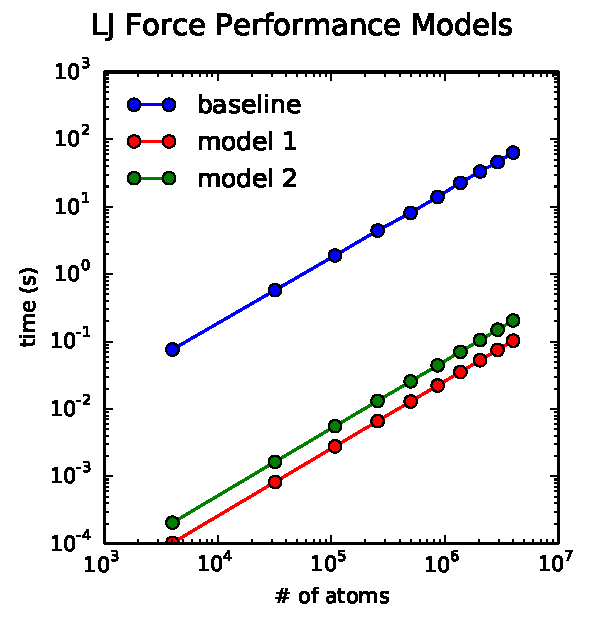
\includegraphics[width=0.5\textwidth]{../figs/perfmodel_forceLJ}
  \caption{Performance models and baseline results. Model 1 is
    equation \ref{eqn:perf-model} with $n=69$ and model 2 is
    \ref{eqn:perf-model} with $n=2\times69$.}
  \label{fig:perf-models}
\end{figure}

\section{Modifications}

The performance baseline revelead a large discrepancy between our
performance model and experimental results. We began to diagnose 

The first thing we noticed while analyzing the source code is a large
number of pointer dereferences to access the arrays storing particle
information. From the code report generated by the Cray compiler it
was clear that these dereferences were being done everytime the
pointers were accessed in the innermost loop of the force
calcuation. A simple optimzation was then to derefernce these pointers
before the computation. The small loops over real3 variables are also
not unrolled by compiler, so we did this by hand. The inner loop of
the force calculation routine is shown before and after optimization
in appendix \ref{apd:code-changes}.

The Cray compiler reports tell us that no vectorization is occuring in
the force calculation. After investgating we determined that this is
in fact the correct behavior, as the data structure used does not
guarantee that the arrays used are not aliased. All particle
information is stored in contigous arrays and aliasing occurs when
calculating the interactions between particles in the same cell. We
considered modifiying the data structure to remove aliasing, but
determined that the modifications required are beyond the scope of
this project.

Another potential improvement considered was changing the order of
particles within a cell to improve memory access patterns. The code
currently sorts the particles within a cell regularly. Because of this
it is unlikely that substational improvements could be made.

After the above modification were made the runtimes using the Cray
compiler were still several orders of magnitude higher than our
performance expectations. With no clear reason for this discrepency we
ran our single core bencharks using code compiled with gcc and found
that the runtime decreased dramatically. From the gcc compiler report
it was clear that no additional vectorization was occuring. We have
been unable to determine the reason for the large difference between
compilers.


\section{Conclusion}
% REFERENCES???



\appendix
\section{Code changes}
\label{apd:code-changes}
The changes made to the inner loop in the force cacluation are shown
here.
\subsection{Initial Inner Force Loop}
\begin{lstlisting}
  real_t dr[3];
  int jId = s->atoms->gid[jOff];  
  if (jBox < s->boxes->nLocalBoxes && jId <= iId )
  continue; // don't double count local-local pairs.
  real_t r2 = 0.0;
  for (int m=0; m<3; m++)
  {
    dr[m] = s->atoms->r[iOff][m]-s->atoms->r[jOff][m];
    r2+=dr[m]*dr[m];
  }

  if ( r2 > rCut2) continue;

  r2 = 1.0/r2;
  real_t r6 = s6 * (r2*r2*r2);
  real_t eLocal = r6 * (r6 - 1.0) - eShift;
  s->atoms->U[iOff] += 0.5*eLocal;
  s->atoms->U[jOff] += 0.5*eLocal;

  if (jBox < s->boxes->nLocalBoxes)
  ePot += eLocal;
  else
  ePot += 0.5 * eLocal;

  real_t fr = - 4.0*epsilon*r6*r2*(12.0*r6 - 6.0);
  for (int m=0; m<3; m++)
  {
    s->atoms->f[iOff][m] -= dr[m]*fr;
    s->atoms->f[jOff][m] += dr[m]*fr;
  }
\end{lstlisting}

\subsection{Optimized Inner Force Loop}
\begin{lstlisting}
  real_t dr[3];
  int jId = gid[jOff];  
  if (jBox < nLocalBoxes && jId <= iId )
  continue; // don't double count local-local pairs.

  real_t r2 = 0.0;
  dr[0] = r_iOff[0]-r[jOff][0];
  r2+=dr[0]*dr[0];
  dr[1] = r_iOff[1]-r[jOff][1];
  r2+=dr[1]*dr[1];
  dr[2] = r_iOff[2]-r[jOff][2];
  r2+=dr[2]*dr[2];

  if ( r2 > rCut2) continue;

  r2 = 1.0/r2;
  real_t r6 = s6 * (r2*r2*r2);
  real_t eLocal = r6 * (r6 - 1.0) - eShift;
  U[iOff] += 0.5*eLocal;
  U[jOff] += 0.5*eLocal;

  if (jBox < nLocalBoxes)
  ePot += eLocal;
  else
  ePot += 0.5 * eLocal;

  real_t fr = - 4.0*epsilon*r6*r2*(12.0*r6 - 6.0);
  f_iOff[0] -= dr[0]*fr;
  f[jOff][0] += dr[0]*fr;
  f_iOff[1] -= dr[1]*fr;
  f[jOff][1] += dr[1]*fr;
  f_iOff[2] -= dr[2]*fr;
  f[jOff][2] += dr[2]*fr;
\end{lstlisting}

\end{document}
